\section{Result}
\label{result}

To compare the results shown in the article \cite{liu2010}, we test our implementation for all the cases reported in that article. All the tests reported below are executed on Pianosa\footnote{Pianosa web site: \url{http://pianosa.di.unipi.it/Home_pianosa/html/info.html}}, the Computer Science Department's Cluster in Pisa. The cluster is composed by 24 homogeneous nodes. The nodes are 800 Mz Pentium III with 1GB of main memory and they are connected together through a Fast Ethernet interconnection network. On that cluster, we installed an Hadoop 0.20.2 framework. The configuration parameters are set to default, so, the maximum number of task per node is set to 2 and the number of replication is set to 3. In our configuration, we decide to place the secondary node and the job traker in cluster interface node that is not used also as task tracker. Only other 21 nodes are available as slave, cause to momentarily unavailability of the other nodes.

The data used in the test are generated by two generators written in Matlab: one for the matrix A and other one for the matrices W and H. Both generators produce positive elements Gaussian distributed. The first one is a sparse matrix generator and its sparsity factor can be tuned through an input parameter. The second one, instead, is a complete matrix generator. For our tests, we fix the $m$ and $n$ parameters respectively to 105000 and 20000.

The first test battery done tests how the computation scales in relation to the the size of the data submitted. 

In the first test executed, the number of non-zero elements in the sparse matrix is changed between $5000000$ and $80000000$ elements while the k parameter remain fixed to 10. The test is executed with 


The reduce task number is set to $ 1,8 * number\_of\_worker$, where is possible\footnote{Note: the phase 3 and 4 have a fixed number of reduce task}. Hadoop User Guide suggest to set the reduce task number to $$ mapred.map/reduceMaximumTask * number\_of\_worker * k $$ where k is a constant choose in the range $[ 0.9, 1.8]$.


The External Phase classes that convert the input data from text to sequence allow to specify how many reducer use. In this way, before the iterative algorith starts we can set the rigth number of input split.



\begin{figure}[th]
	\centerline{
		\mbox{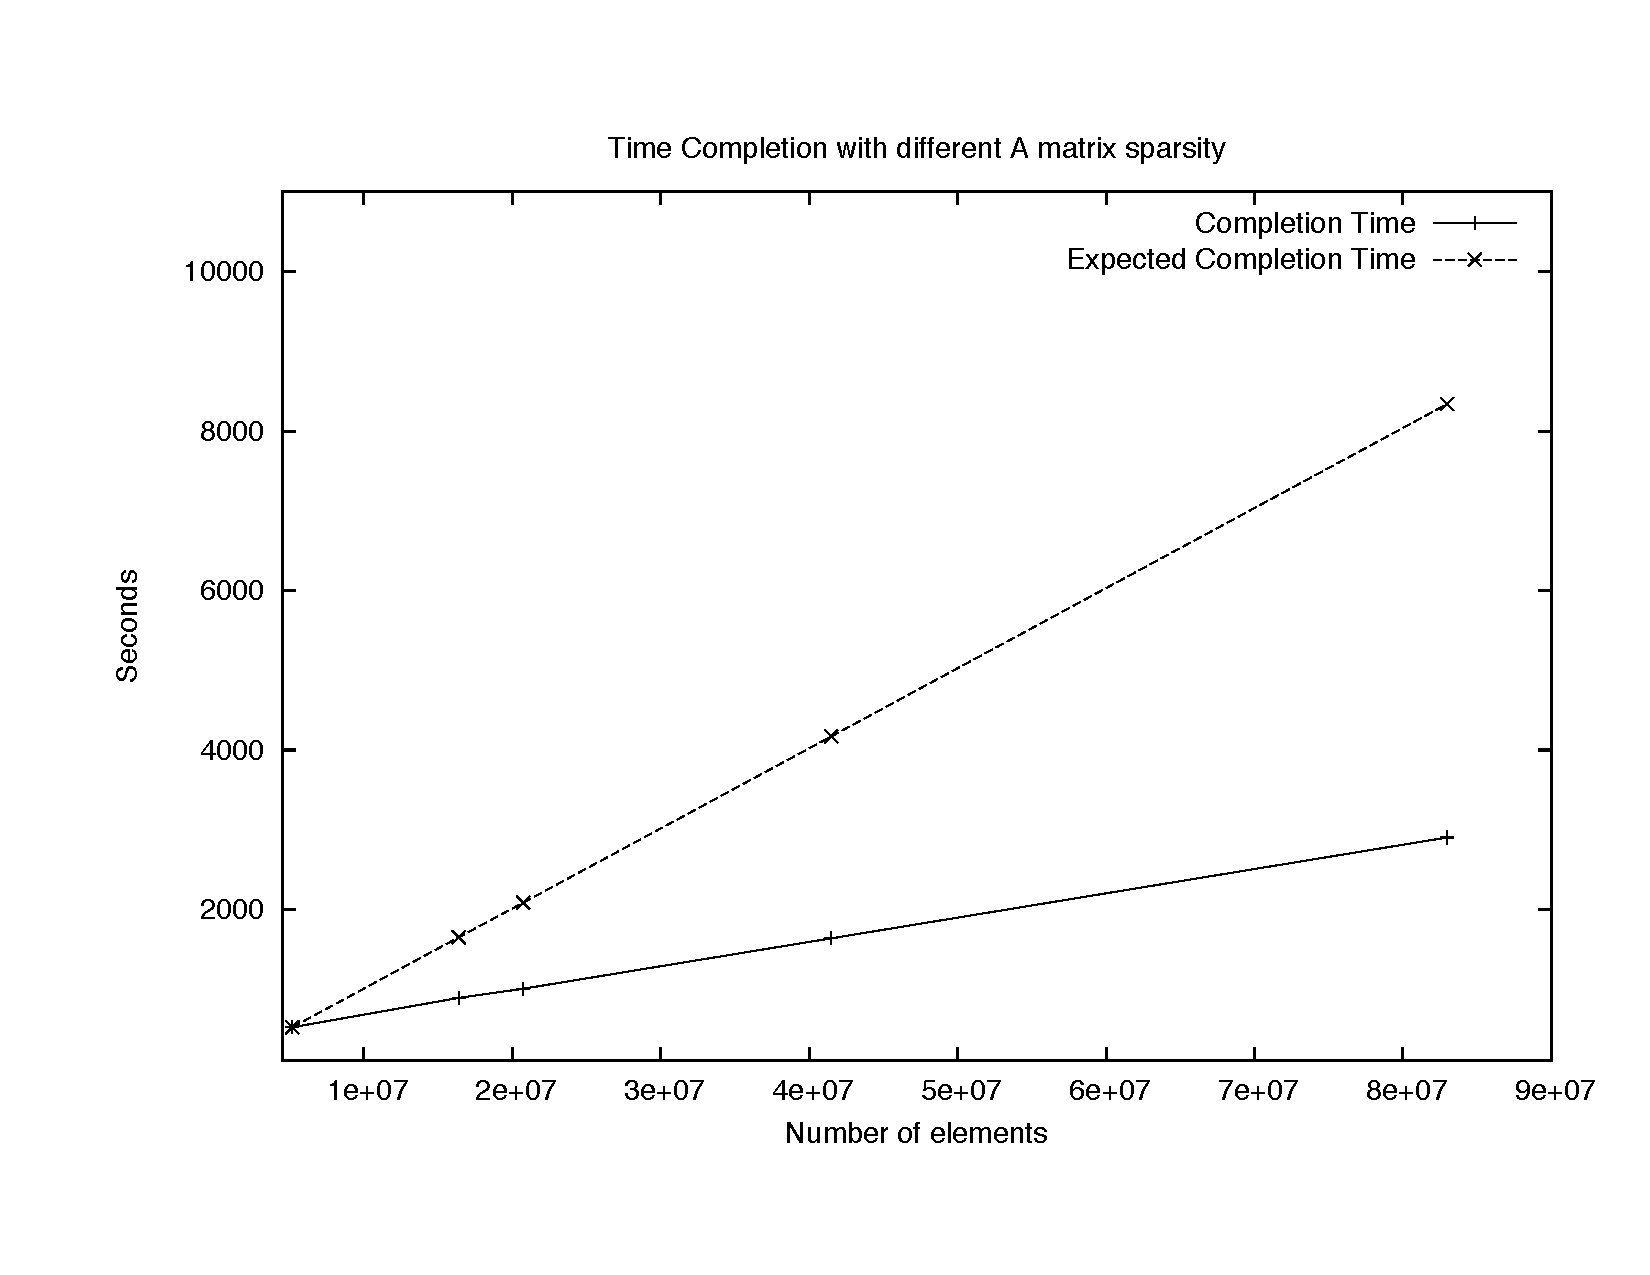
\includegraphics[scale=0.45]{HadoopTest/PsFiles/DeltaVar.pdf}}
	}
	\caption{Comparazione tra le forme di parallelismo del caso di studio 3 al variare del grado di parallelismo} 
\end{figure}

\begin{figure}[th]
	\centerline{
		\mbox{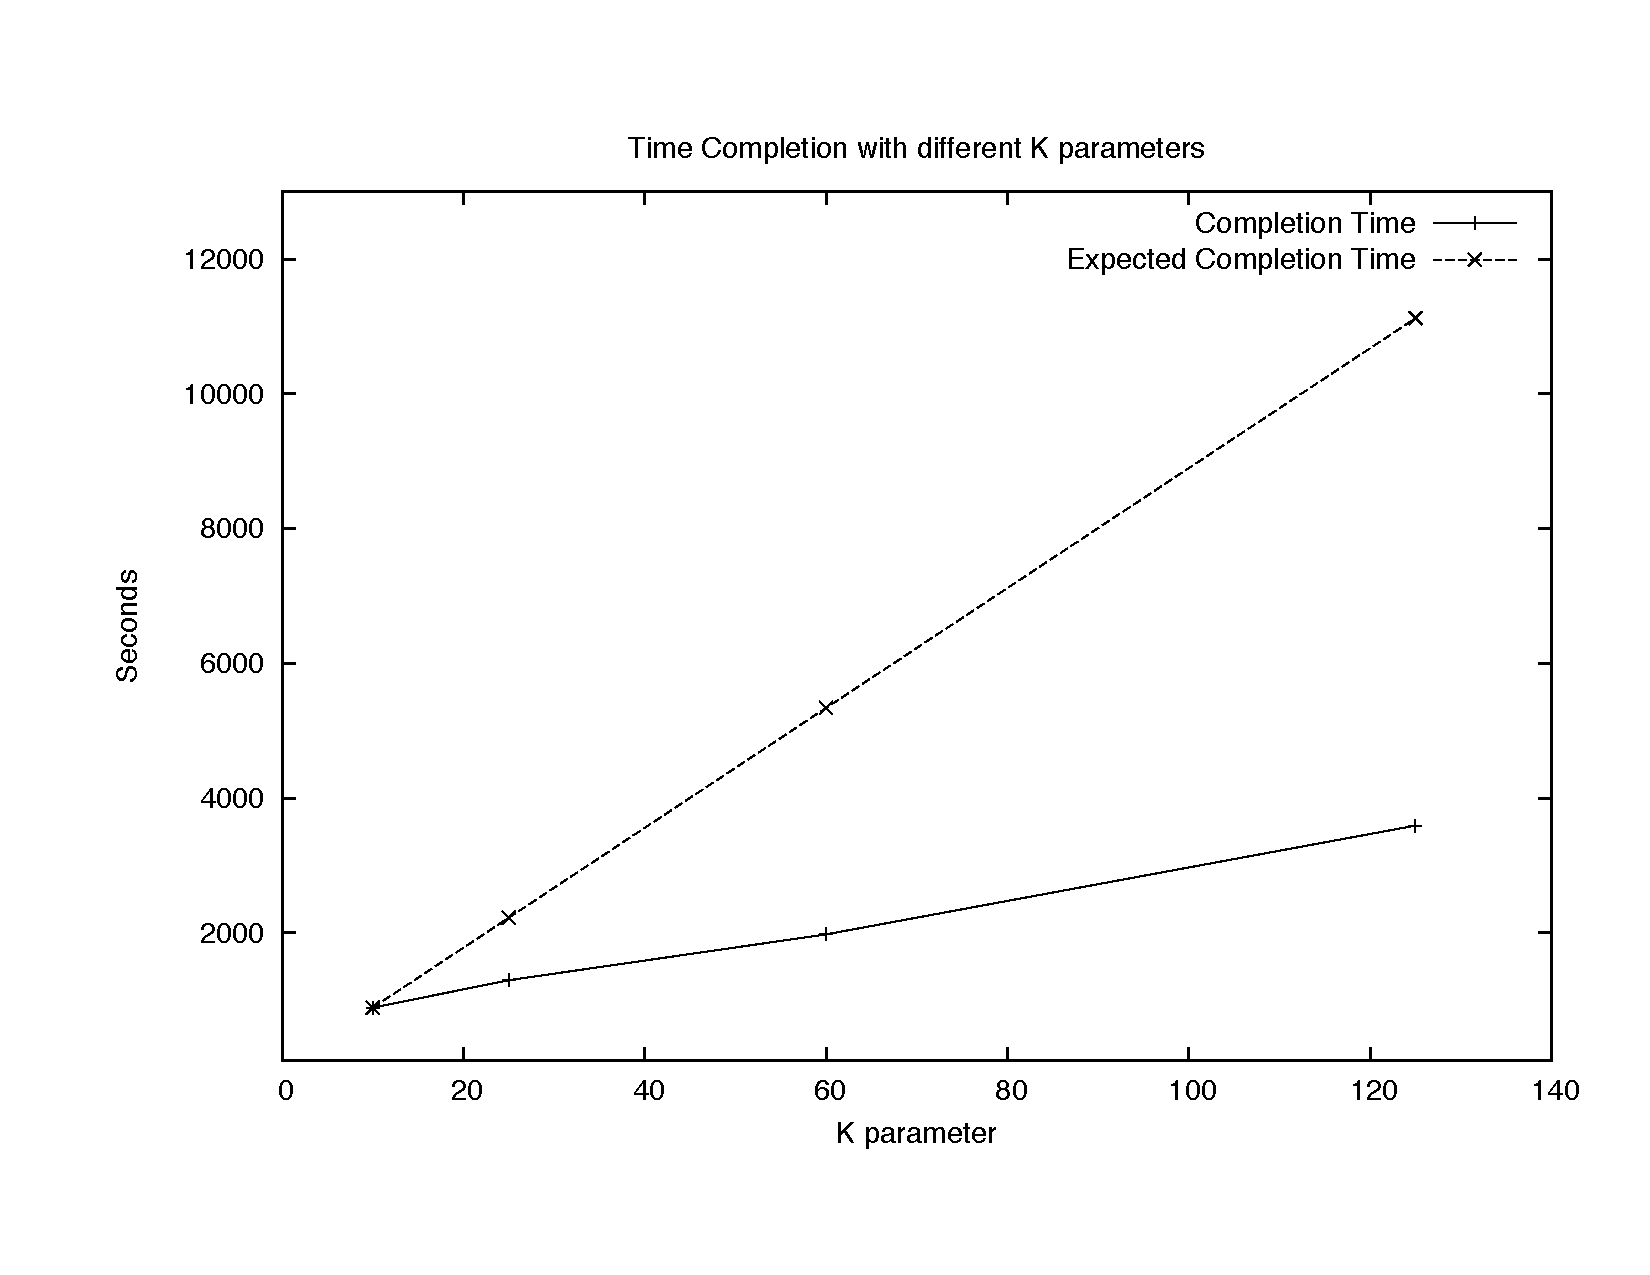
\includegraphics[scale=0.45]{HadoopTest/PsFiles/kVar.pdf}}
	}
	\caption{Comparazione tra le forme di parallelismo del caso di studio 3 al variare del grado di parallelismo} 
\end{figure}

\begin{figure}[th]
	\centerline{
		\mbox{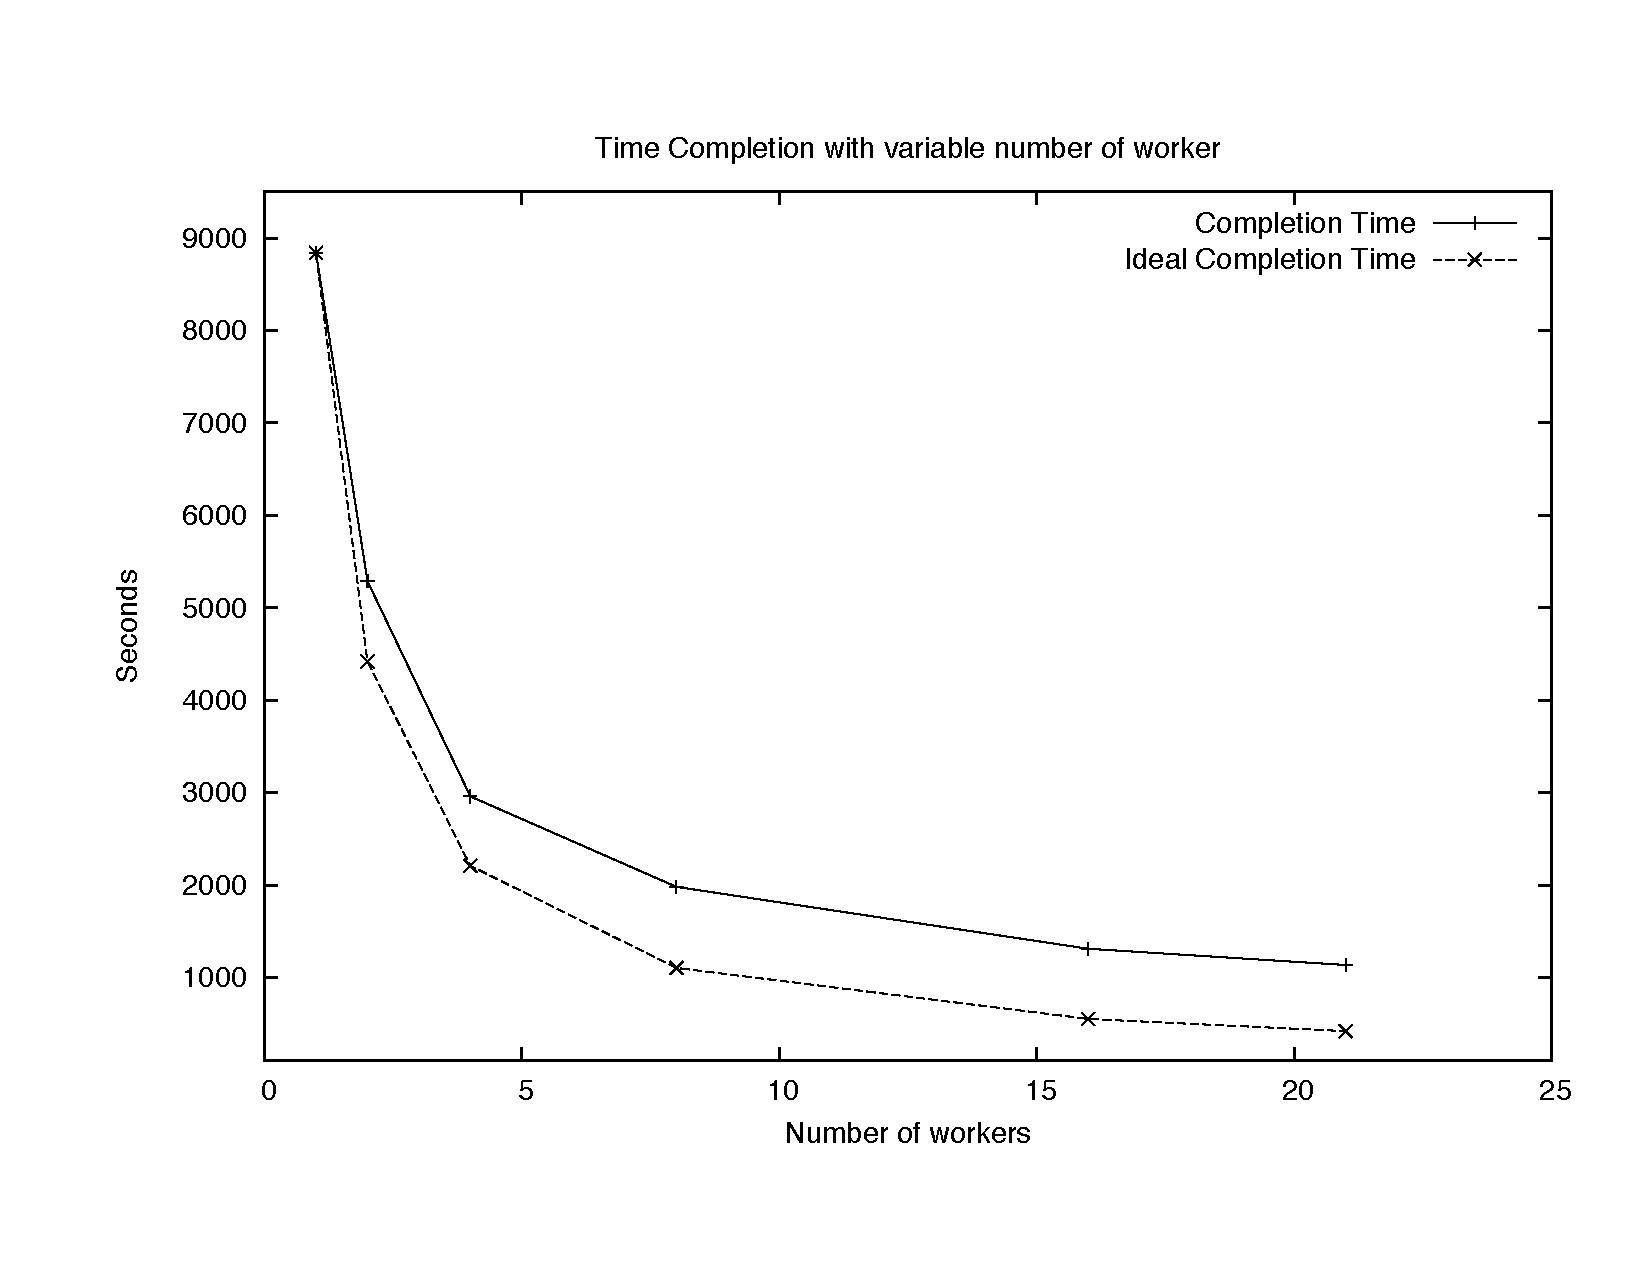
\includegraphics[scale=0.45]{HadoopTest/PsFiles/NTime.pdf}}
	}
	\caption{Comparazione tra le forme di parallelismo del caso di studio 3 al variare del grado di parallelismo} 
\end{figure}

\begin{figure}[th]
	\centerline{
		\mbox{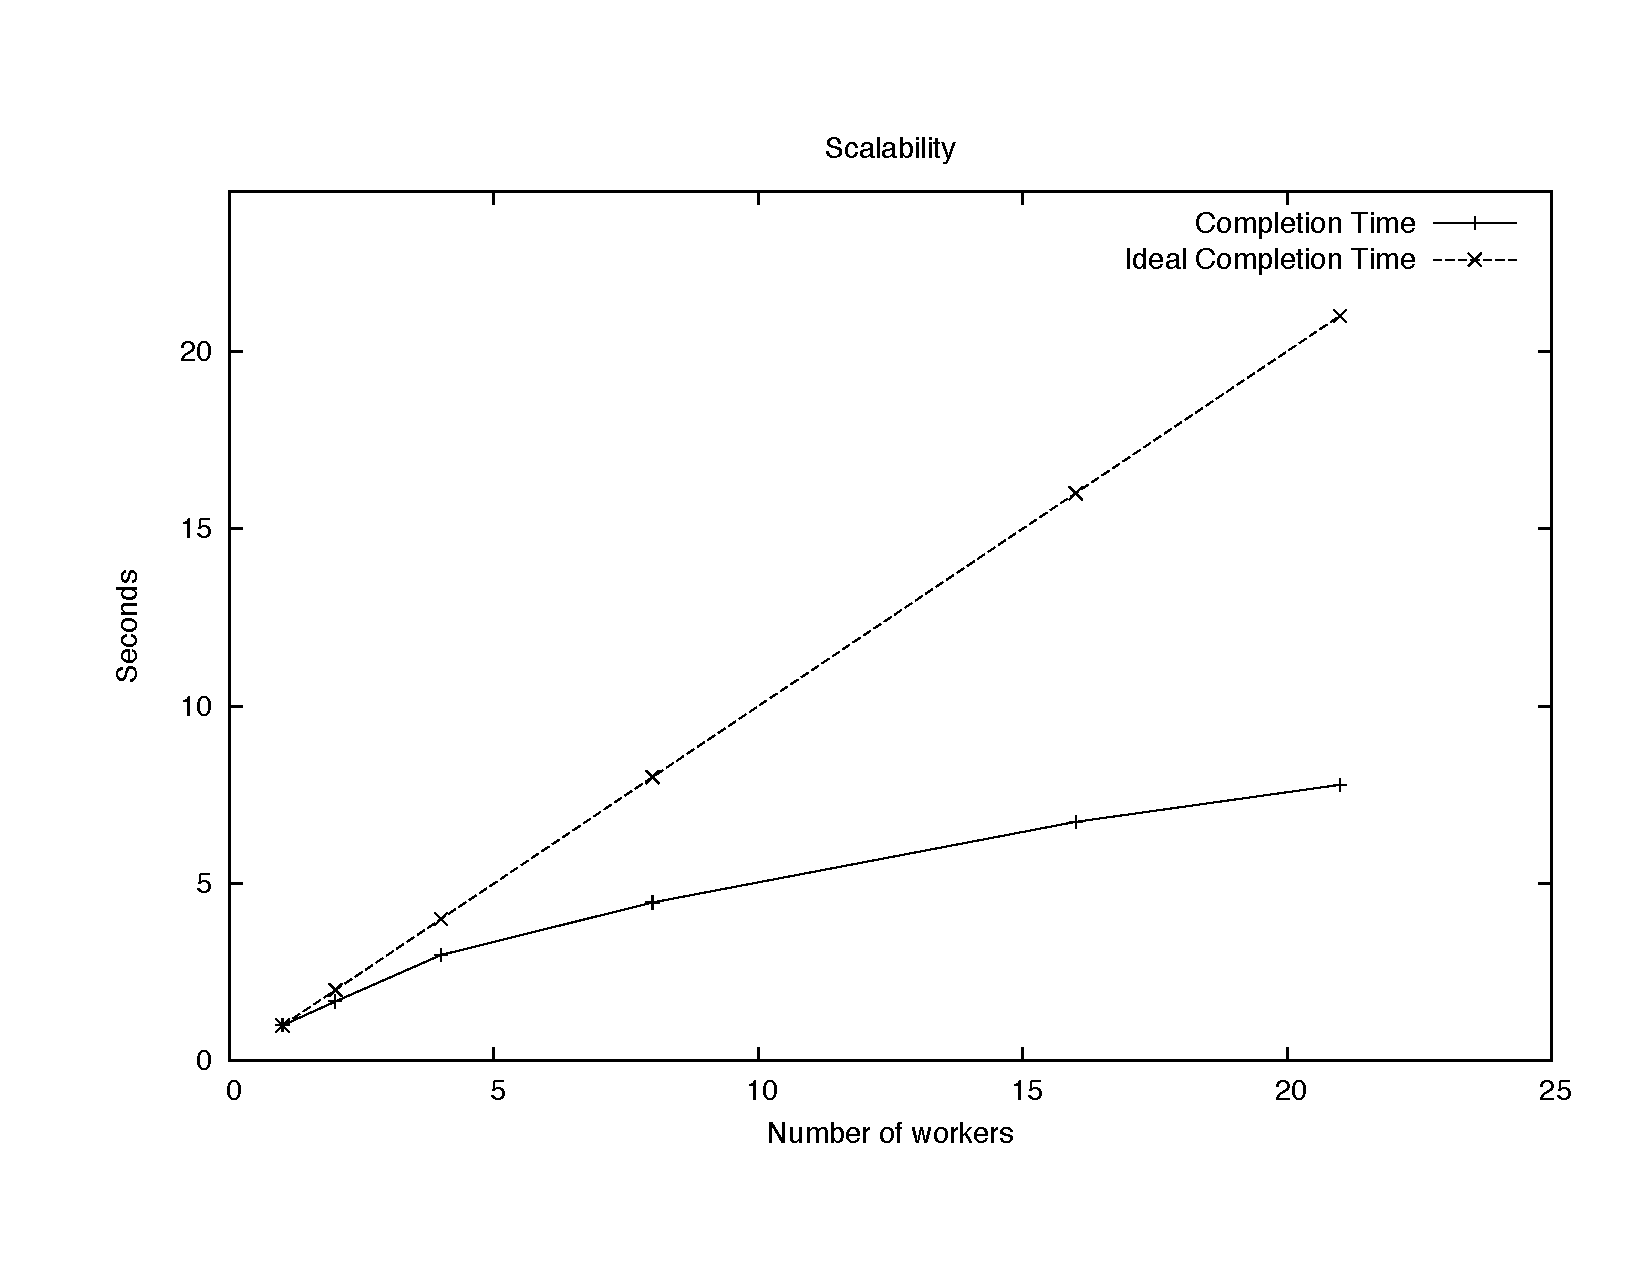
\includegraphics[scale=0.45]{HadoopTest/PsFiles/NScal.pdf}}
	}
	\caption{Comparazione tra le forme di parallelismo del caso di studio 3 al variare del grado di parallelismo} 
\end{figure}
